\subsection{Alignment Training}

\begin{frame}
\subsectionpage
\end{frame}

\begin{frame}{Alignment Training}
   
    \resizebox{\textwidth}{!}{
    \begin{tikzpicture}
   \draw[mLightBrown!30] (6.2,0) -- (6.2,-8.15);
   \uncover<4-5>{
   \draw[mLightBrown!30] (6.2,0) -- (6.2,-9.21);
   }
   \draw[mLightBrown!30] (0,0) -- (0,-4.85);

   \uncover<1-5>{
       \node[align=left,text width=10cm,anchor=north west] at (0,0) {\texttt{{\color{mLightBrown}\# Input}\\x = [\\~\\~\\~\\~\\~\\~\\]}};
   }
   \uncover<1-2>{
       \node[anchor=west] at (0.5,-2.8) 
       {\resizebox{5.5cm}{!}{$\pi\left( \left[\!\!\!\left[ \begin{array}{l}
        \textsc{Inform}\\
        \textrm{\only<2>{\color{Red}}name=Aromi}\\
        \textrm{\only<2>{\color{Green}}eat\_type=coffee shop}\\
        \textrm{\only<2>{\color{Blue}}area=city centre}\\
    \end{array}\right]\!\!\!\right]\right)$ }};


   }
\uncover<2>{
    \draw[line width=1.5mm,draw=Green,<->] (5.4,-3.1) to [out=0,in=270] (6.15,-2.8) to [out=90,in=180] (6.8,-2.5);
\node at (4.25,-2.55) {};
    \draw[line width=1.5mm,draw=Red,<->] (4.20,-2.55) to [out=0,in=90] (6.15,-3.10) to [out=270,in=180] (6.70,-6.36);
    \draw[line width=1.5mm,draw=Blue,<->] (4.70,-3.56) to [out=0,in=180] (6.70,-4.36);
}
\uncover<3>{
    \draw[line width=1.5mm,draw=Green,<->] (5.2,-2.5) to [out=0,in=180] (6.8,-2.5);
\node at (4.25,-2.55) {};
    \draw[line width=1.5mm,draw=Red,<->] (3.20,-3.55) to [out=0,in=180] (6.70,-6.36);
    \draw[line width=1.5mm,draw=Blue,<->] (4.40,-3.0) to [out=0,in=180] (6.70,-4.36);
}
\uncover<5>{
    \draw[line width=1.5mm,draw=Green,<->] (5.2,-2.5) to [out=0,in=180] (6.8,-3.7);
\node at (4.25,-2.55) {};
    \draw[line width=1.5mm,draw=Red,<->] (3.20,-3.00) to [out=0,in=90] (5.85,-4.08) to [out=270,in=180] (6.70,-5.16);
    \draw[line width=1.5mm,draw=Blue,<->] (4.40,-3.55) to [out=0,in=180] (6.70,-7.06);
}

   \uncover<3>{
       \node[align=left,text width=10cm,anchor=north west] at (0,0) {\texttt{{\color{mLightBrown}\# Input}\\x = [\\
                    ~~~~"<<s>>",\\
                ~~~~"inform",\\
                ~~~~{\color{Green}"eat\_type=coffee shop",}\\
                ~~~~{\color{Blue}"area=city centre",}\\
                ~~~~{\color{Red}"name=Aromi",}\\
                ~~~~"<<e>>"\\
            ]\\~
   }};
}
   \uncover<5>{
       \node[align=left,text width=10cm,anchor=north west] at (0,0) {\texttt{{\color{mLightBrown}\# Input}\\x = [\\
                    ~~~~"<<s>>",\\
                ~~~~"inform",\\
                ~~~~{\color{Green}"eat\_type=coffee shop",}\\
                ~~~~{\color{Red}"name=Aromi",}\\
                ~~~~{\color{Blue}"area=city centre",}\\
                ~~~~"<<e>>"\\
            ]\\~
   }};
}
   \uncover<1-3>{
         \node[align=left,text width=5.75cm,anchor=north west] at (6.2,0) {\texttt{{\color{mLightBrown}\# Output}\\y = [\\ 
                    ~~~~"<<s>>",\\ 
                    ~~~~"for",\\
                    ~~~~\only<1>{"coffee",}\only<2->{{\color{Green}"coffee",}}\\
                    ~~~~"in",\\
                    ~~~~"the",\\
                ~~~~{\only<2->{\color{Blue}}"city",}\\
            ~~~~{\only<2->{\color{Blue}}"centre",}\\
                    ~~~~",",\\
                    ~~~~"try",\\
                ~~~~{\only<2->{\color{Red}}"aromi",}\\
                    ~~~~".",\\
                    ~~~~"<<e>>"\\
                ] \\ ~
   }};
   }

   \uncover<4-5>{
         \node[align=left,text width=5.75cm,anchor=north west] at (6.2,0) {\texttt{{\color{mLightBrown}\# Output}\\y = [\\ 
                    ~~~~"<<s>>",\\ 
                    ~~~~"there",\\
                    ~~~~"is",\\
                    ~~~~"a",\\
                    ~~~~{{\color{Green}"coffee",}}\\
                    ~~~~{{\color{Green}"shop",}}\\
                    ~~~~"called",\\
                ~~~~{\color{Red}"aromi",}\\
                    ~~~~"in",\\
                    ~~~~"the",\\
                ~~~~{\color{Blue}"city",}\\
            ~~~~{\color{Blue}"centre",}\\
                    ~~~~".",\\
                    ~~~~"<<e>>"\\
                ] \\ ~
   }};
   }


   \uncover<2->{
   \node[text width=5cm,anchor=north west] at (0,-5) {\begin{enumerate} \item Align utterance \texttt{y} to attribute-values. \item<3-> Order \texttt{x} according to the order the attribute-values are realized in \texttt{y}.\end{enumerate}};
   }
    \end{tikzpicture}
}
\end{frame}

\begin{frame}{Alignment Training Yields Controllable Generation}
  \begin{center}
    \resizebox{1.0\textwidth}{!}{
    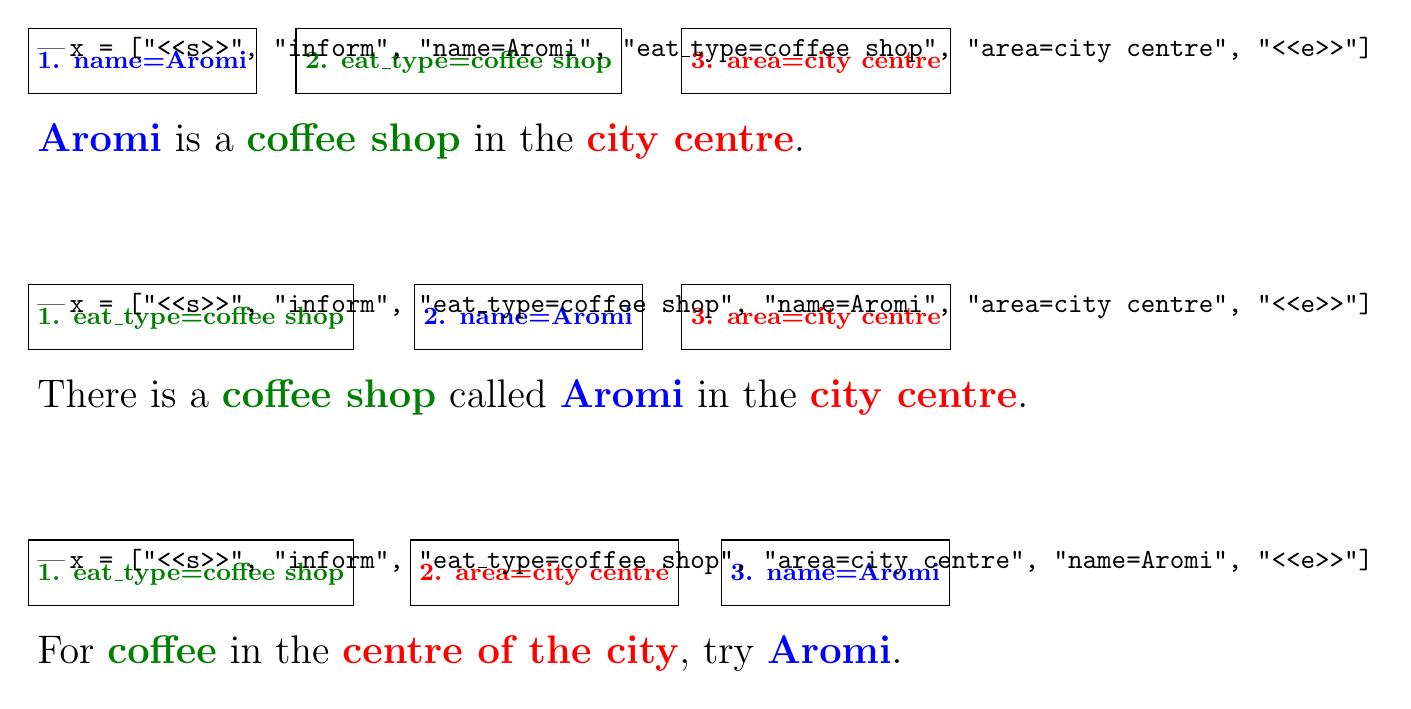
\begin{tikzpicture}[
        plan/.style = {draw,anchor=north west,minimum height=0.75cm,
                       font=\small,text height=0.4cm,text depth=0.2cm},
        plan.name/.style = {plan,text=Blue},
        plan.eat/.style = {plan,text=Green},
        plan.area/.style = {plan,text=Red},
        input/.style = {anchor=north west}]

      \def\plY{3.25};

      \uncover<1>{
        \node[plan.name] at (0.0, 3*\plY) {\textbf{1. name=Aromi}};
        \node[plan.eat]  at (3.4, 3*\plY) {\textbf{2. eat\_type=coffee shop}};
        \node[plan.area] at (8.3, 3*\plY) {\textbf{3. area=city centre}};
      }
      \uncover<2->{
        \node[input] at (0.0, 3*\plY) 
        {\alert{|$\,$}\texttt{x = ["<<s>>",
                          "inform", 
                          "name=Aromi", 
                          "eat\_type=coffee shop", 
                          "area=city centre",
                          "<<e>>"]}};

      }

      \node[anchor=north west] at (0,3*\plY-1.1) {\Large {\color{Blue}\uline{\textbf{Aromi}}} is a {\color{Green}\uline{\textbf{coffee shop}}} in the {\color{Red}\uline{\textbf{city centre}}}.};

      \uncover<1-2>{
        \node[plan.eat]  at (0.0,2*\plY) {\textbf{1. eat\_type=coffee shop}};
        \node[plan.name] at (4.9,2*\plY) {\textbf{2. name=Aromi}};
        \node[plan.area] at (8.3,2*\plY) {\textbf{3. area=city centre}};
      }
      \uncover<3->{
        \node[input] at (0.0,2*\plY) 
            {\alert{|$\,$}\texttt{x = ["<<s>>",
                          "inform",  
                          "eat\_type=coffee shop", 
                          "name=Aromi",
                          "area=city centre",
                          "<<e>>"]}};
      }
        
      \node[anchor=north west] at (0,2*\plY-1.1) {\Large There is a {\color{Green}\uline{\textbf{coffee shop}}} called {\color{Blue}\uline{\textbf{Aromi}}} in the {\color{Red}\uline{\textbf{city centre}}}.} ;

      \uncover<1-3>{
        \node[plan.eat]  at (0.0,1*\plY) {\textbf{1. eat\_type=coffee shop}};
        \node[plan.area] at (4.85,1*\plY) {\textbf{2. area=city centre}};
        \node[plan.name] at (8.8,1*\plY) {\textbf{3. name=Aromi}};
      }
      \uncover<4>{
        \node[input] at (0.0,1*\plY) 
            {\alert{|$\,$}\texttt{x = ["<<s>>",
                          "inform",  
                          "eat\_type=coffee shop", 
                          "area=city centre",
                          "name=Aromi",
                          "<<e>>"]}};
      }
        \node[anchor=north west] at (0,1*\plY-1.1) {\Large For {\color{Green}\uline{\textbf{coffee}}} in the {\color{Red}\uline{\textbf{centre of the city}}}, try {\color{Blue}\uline{\textbf{Aromi}}}.} ;



    \end{tikzpicture}
}
        \end{center}

\end{frame}
